\documentclass[a5paper,twoside,11pt]{report}

%%%%%%%%%% Packages %%%%%%%%%%
\usepackage[outer=2cm, inner=2cm, bottom=2.5cm]{geometry}
\usepackage[bottom]{footmisc} 
\usepackage{hiero}
\usepackage{egypto}
\usepackage[backend=biber, style=authoryear-icomp, block=ragged]{biblatex}
\usepackage{longtable}
\usepackage{fancyhdr}
\usepackage{microtype}
\usepackage{graphicx}
\usepackage{wrapfig}
\usepackage{enumitem}
\usepackage{amsmath}
%\usepackage[utf8]{inputenc}
\usepackage{fontspec}
\usepackage[greek,english]{babel} 
\usepackage{epigraph}
\usepackage{lmodern}
\usepackage{afterpage}
\usepackage{nonumonpart}
\usepackage{titlesec}
\usepackage{microtype}
\usepackage{titling} 
\usepackage[T1]{fontenc}
\usepackage{bold-extra}
\usepackage{listings}
\usepackage{xcolor}
\usepackage{libertine}
\linespread{1.1}
\raggedbottom

% \usepackage{draftwatermark}
\makeindex



%Some Hieroglyph stuff
\newcommand{\AHiero}{{\fontspec{DejaVu Sans}Ꜣ}}
\newcommand{\aHiero}{{\fontspec{DejaVu Sans}ꜥ}}
\newcommand{\xHiero}{ḫ}
\newcommand{\XHiero}{ẖ}
\newcommand{\HHiero}{ḥ}
\newcommand{\DHiero}{ḏ}
\newcommand{\THiero}{ṯ}
\newcommand{\SHiero}{š}
\newcommand{\qHiero}{ḳ}

\addbibresource{bibliography.bib}
\TextHieroglyphs

% \SetWatermarkText{Preview}
\newlength\longest
\setlength{\marginparwidth}{0pt}
\setlength{\headheight}{15pt}

\titleformat{\section}[wrap]
{\normalfont\bfseries}
{\thesection.}{0.5em}{}
\titlespacing{\section}{12pc}{1.5ex plus .1ex minus .2ex}{1pc}

\definecolor{backcolor}{rgb}{0.95,0.95,0.92}

\lstdefinestyle{mystyle}{
      backgroundcolor=\color{backcolor},
      basicstyle=\ttfamily\footnotesize,
      breakatwhitespace=false,         
      breaklines=true,                 
      captionpos=b,                    
      keepspaces=true,                 
      numbers=left,                    
      numbersep=5pt,                  
      showspaces=false,                
      showstringspaces=false,
      showtabs=false,                  
      tabsize=2
}
\lstset{style=mystyle}
%%%%%%%%%% Fancy HDR %%%%%%%%%%
\pagestyle{fancy}
\fancyhf{}
\fancyhead[LE,RO]{\thepage}
\fancyhead[LO]{\nouppercase{\leftmark}}
\fancyhead[RE]{\textsc{The Intricacies of Ancient Egyptian Hieroglyphics}}
\fancypagestyle{plain}{
\fancyhf{} 
\fancyhead[LE,RO]{\thepage}
\fancyhead[LO]{\leftmark}
\fancyhead[RE]{\textsc{The Intricacies of Ancient Egyptian Hieroglyphics}}}

\begin{document}
\pagenumbering{gobble} 

%%%%%%%%%% Pretitle %%%%%%%%%%
\thispagestyle{empty}
\begin{center}
	\includegraphics[scale=0.162]{cover.png}
\end{center}
\newpage

%%%%%%%%%% EMPTY PAGE %%%%%%%%%% 
\thispagestyle{empty}
  \mbox{}
  \newpage

%%%%%%%%%% Posttitle %%%%%%%%%% 
\title{%
  The Intricacies of Ancient Egyptian Hieroglyphics\\
  \begin{center}
    \textit{Learning the basics of the Ancient Egyptian writing system; for complete beginnners}
  \end{center}
}
\author{By Marvin Johanning}
\date{}
\maketitle

%%%%%%%%%% Copyright and Impressum %%%%%%%%%%
\thispagestyle{empty}
\noindent\textsc{\underline{Text}}: © Copyright 2020 Marvin Johanning

\noindent\textsc{\underline{Cover design}}: © Copyright 2020 Marvin Johanning

\noindent© 2020 by Marvin Johanning\\``The Intricacies of Ancient Egyptian Hieroglyphics: Learning the basics of the Ancient Egyptian writing systems; for complete beginners'' by Marvin Johanning is licensed under CC BY-NC-SA 4.0. To view a copy of this license, visit https://creativecom\\mons.org/licenses/by-nc-sa/4.0.

\vspace{10mm}\noindent\textsc{Publishing}: \\
Marvin Johanning\\
Salzufler Str. 66\\
33719 Bielefeld\\
info@marvinjohanning.de

\vspace{5mm}\noindent\textsc{Printing}: epubli – ein Service der neopubli GmbH, Berlin
\newpage

%%%%%%%%%% Introductory quote %%%%%%%%%%
\clearpage
\thispagestyle{empty}
\begin{center}
\DisplayHieroglyphs
\begin{hieroglyph}{\leavevmode \LoneHorizontalLine{\loneSign{\Aca GM/48/}\HinterSignsSpace
\loneSign{\Aca GG/77/}}\HinterSignsSpace
\Cadrat{\CadratLineI{\Aca GO/65/}\CadratLine{\Aca GN/69/}}\HinterSignsSpace
\loneSign{\Aca GY/35/}\HinterSignsSpace
\loneSign{\Aca GN/66/}\HinterSignsSpace
\loneSign{\Aca GA/32/}\HinterSignsSpace
\loneSign{\Aca GG/50/}\HinterSignsSpace
\loneSign{\Aca GU/60/}\HinterSignsSpace
\Cadrat{\CadratLineI{\Aca GX/32/}\CadratLine{\Aca GY/32/}}\HinterSignsSpace
\Cadrat{\CadratLineI{\Aca GX/32/}\CadratLine{\Aca GN/66/}}\HinterSignsSpace
\Cadrat{\CadratLineI{\Aca GN/66/}\CadratLine{\Aca GE/41/}}\HinterSignsSpace
\loneSign{\Aca GG/77/}\HinterSignsSpace
\loneSign{\Aca GE/46/}\HwordSpace
\loneSign{\Aca GU/37/}\HinterSignsSpace
\LoneHorizontalLine{\loneSign{\Aca GM/48/}\HinterSignsSpace
\loneSign{\Aca GM/48/}}\HinterSignsSpace
\loneSign{\Aca GA/32/}\HinterSignsSpace
\Cadrat{\CadratLineI{\Aca GN/66/}\CadratLine{\Aca GZ/37/}}\HinterSignsSpace
\Cadrat{\CadratLineI{\Aca GAa/43/}\CadratLine{\Aca GG/70/}}\HwordSpace
\loneSign{\Aca GF/66/}\HinterSignsSpace
\Cadrat{\CadratLineI{\Aca GI/41/}\CadratLine{\Aca GD/52/}}\HinterSignsSpace
\LoneHorizontalLine{\loneSign{\Aca GG/77/}\HinterSignsSpace
\loneSign{\Aca GZ/37/}}\HinterSignsSpace
\Cadrat{\CadratLineI{\Aca GV/44/}\CadratLine{\Aca GN/66/}}}\end{hieroglyph}
\null\vfill
\vfill\vfill
\clearpage\newpage
\end{center}
\newpage

%%%%%%%%%% Table of Contents %%%%%%%%%%
\tableofcontents
\newpage

%%%%%%%%%% Introduction %%%%%%%%%%
\pagenumbering{roman}
\chapter*{Preface to second edition}
  \markboth{Preface to second edition}{Preface to second edition}
  \addcontentsline{toc}{chapter}{Preface to second edition}
	CONTENT HERE

	\newpage

	%%%%%%%%%% About %%%%%%%%%%
	\chapter*{About me}
		\markboth{About me}{About me}
		\addcontentsline{toc}{chapter}{About me}

		My name is Marvin Johanning, I am twenty-one years old and currently reside in a city many deem to not exist — which, obviously, is untrue for I \textit{do} live here and surely I am real. I like writing things even though, perhaps, I am not great at it; yet I enjoy doing so and only through practice can you improve, which is why I write as much as possible as frequently as I can.

		I have recently switched from writing in LibreOffice to \LaTeX, as LibreOffice has proven itself to be headache-inducing when working with large amounts of text which you wish to reformat at a later date. 

		I tend to write about things relating to languages — be it real or programming languages —, computers and, though rarely, politics. All of these can be found on my website. My biggest writing project to-date is \textit{The Intricacies of Ancient Egyptian Hieroglyphics} (ISBN: 978-3-752952-49-0), which incidentally, was what led me to use \LaTeX, information regarding which can, too, be found on my website.
		\newpage


%%%%%%%%%% Empty page %%%%%%%%%%
\pagenumbering{gobble}
\thispagestyle{empty}
  \mbox{}
  \newpage

%%%%%%%%%% Beginning of text itself %%%%%%%%%%
\pagenumbering{arabic}
\part*{History and general information}
\markboth{History and general information}{History and general information}
\addcontentsline{toc}{part}{History and general information}
  \newpage

\thispagestyle{empty}
  \mbox{}
  \newpage

\chapter*{Who deciphered the Hieroglyphs?}
  \markboth{Who deciphered the Hieroglyphs?}{Who deciphered the Hieroglyphs?}
  \addcontentsline{toc}{chapter}{Who deciphered the Hieroglyphs?}
  Before we commence with the study of the script itself, we will begin by talking about how we are even aware of the meaning of the hieroglyphs. Many people will probably cite Jean-François Champollion as being the first to decipher them; and while this is not wrong per se, it paints a slightly wrong picture, and many people believe that no attempts at deciphering the script had been made before him. In actuality, however, there have been many people that, prior to him, have tried their hands at deciphering this fascinating script — one of which was the Arabic alchemist Ibn Wahshiyya who was born in the 9th century CE.

	He was one of the first people to realise the complexity of Egyptian hieroglyphics; yet there is a surprising lack of information about him and his book (Kitab) Shauq Al-Mustaham fi Ma‘irfat Rumuz Al-Aqlam. Even the translation of the title itself seems to be quite a mystery, since I was unable to find a single, proper translation of it. The official English title of the book, written by Joseph Hammer — an Austrian scholar born in the late 18th century whose full name was Joseph von Hammer-Purgstall — in 1806, has the rather unwieldy name of Ancient alphabets and hieroglyphic characters explained; with an Account of the Egyptian priests, their classes, initiation and sacrifices\footnote{And it also seems to me that simply finding a physical copy of the book is difficult. My local university has a quite a considerable book collection and I am usually able to find all the books I need; however, this particular book is only available on microfilm and not as a hard copy. I thus decided to download a digital copy of the book from the Internet Archive.}.

	Upon asking native Arabic speakers however, I have managed to ascertain that the title probably means something along the lines of The Desire to Understand the Meaning of What is Written, which I believe is a rather fitting title; yet, Purgstall’s English version has the original title translated as The long desired Knowledge of occult Alphabets attained, which I find to be a rather dramatic-sounding name. 

	Not only did Ibn Wahshiyya — who, interestingly, is cited as being called Ahmad Bin Abubekr Bin Wahshih in Hammer’s book — actually realise that the Egyptian hieroglyphs are not merely picture writing — a believe still quite prevalent today —, he also discusses and deciphers a great number — more than eighty — of other scripts in his book by giving their equivalents in the Arabic script. It includes the alphabets used by many a philosopher or king and also a number of other alphabets that were in regular use at the time; it is, therefore, in my opinion, a must-read for anyone who is interested in learning about ancient alphabets and ciphers. 

	Knowledge of the Arabic script is recommended in order to understand what sound-value each of the deciphered letters has, but Purgstall's English translation gives a quick overview of them at the beginning of the book. Therefore, we will now be taking a quick look at what he had to say about Egyptian hieroglyphs.

	Firstly, the name given by him to the Egyptian hieroglyphic script is The Hermesian Alphabet \parencite[p. 14]{wahshiyya} which, I believe, is in reference to the Egyptian god Thoth — because the Ancient Greeks generally regarded their god Hermes to be the same as the Egyptian god Thoth — who is, amongst a myriad of other things, known for being the supposed inventor of the Egyptian hieroglyphs and, by extent, writing itself.

	He continues by mentioning that each one of the kings of the Hermesian dynasty invented their own, unique alphabet, derived from commonplace objects, such as plants, people, et cetera \parencite[pp. 14-15]{wahshiyya}. Wahshiyya then lists a rather extensive number of hieroglyphs which he structures into three different series, each one of which relates to a different topic: the first series covers words relating to “Animal Actions and Affections”; the second series covers words relating to “Trees and Plants, and their Produce”; and the third — which, surprisingly, is called the fourth series in this book’s translation — covers words relating to minerals (see photo: “The first Series”, page 114). \parencite[pp. 19-40]{wahshiyya}
	One intriguing aspect of this particular chapter of the book is him mentioning the following: —

	\begin{quote}“… [T]here is a sign which signifies the name of the God Almighty, simply and alone. If they wished to express one of the particular attributes of God, they added something to the original sign, and proceded [sic] in this manner, as you will perceive by the alphabet in question.” \parencite[p. 16]{wahshiyya}\end{quote}

	This is interesting insofar as he clearly must have had at least some understanding of Egyptian hieroglyphs, since this is a concept nowadays usually referred to as determinatives — something we will be discussing more in-depth later —, which most scholars of this time period, and even in the 19th century, did not know of.

	After covering these three series of hieroglyphs we find ourselves in the appendix (Wahshiyya 41–54), in which he continues by examining what he refers to as the Shimshim Alphabet (see photo: “Shimshim Alphabet”, page 115); a number of glyphs discussed and presented therein bare a strong resemblance to Egyptian hieroglyphs, a couple of them being transcribed somewhat accurately. For example, the phonetic value he applies to the hieroglyph \begin{hieroglyph}{\leavevmode \loneSign{\Aca GO/32/}}\end{hieroglyph} is “p”; and this is actually not entirely incorrect, since, in reality, this hieroglyph has the phonetic value “pr” and the meaning of “house”.

	Another hieroglyph he seems to have deciphered semi-accurately is \begin{hieroglyph}{\leavevmode \loneSign{\Aca GQ/32/}}\end{hieroglyph} which he applies the phonetic value of “s” to; and even though it is never used on its own to signify the sound “s”, it is used to represent the sound-sequence “st”\footnote{It seems that it can also stand for the sound sequence “jst”.} and is most commonly used in the name of the god Osiris (\begin{hieroglyph}{\leavevmode \Cadrat{\CadratLineI{\Aca GQ/32/}\CadratLine{\Aca GD/35/}}\HinterSignsSpace
\loneSign{\Aca GA/74/}}\end{hieroglyph}).

	And while his attempt at deciphering this, even back then, ancient language was just that — an attempt —, he was still one of the first people to at least try deciphering them while also realising that the hieroglyphic writing system is not a mere logography\footnote{A writing system wherein one glyph represents a concept, word or entire phrase; often referred to as “picture writing”. A modern-day example of a logographic script is the Chinese writing system, i.e.\ Hanzi.}. 

	It took a reasonably long time before any real attempts at deciphering the Egyptian hieroglyphic script were made again and it all began with Napoleon. During his Egyptian campaign in the late 18th and early 19th century, his troops discovered what is now referred to as the Rosetta Stone. The stele\footnote{A stele is a slab made out of stone or other material (usually wood) intended to be used as a monument.} was originally created in the Ptolemaic dynasty\footnote{This name is not, as you may have thought, related to the Greek mathematician and astronomer Ptolemy, but rather the dynasty of kings (Pharaohs) that was the last to rule Egypt from the 2nd to the end of the 1st century BC.} near the end of 2nd century BC, in around 190 BC. This find would not have been anything particularly exciting, had there not been two languages on it: Ancient Egyptian written in two scripts (hieroglyphic and Demotic\footnote{The Demotic script developed from the Hieratic script which was the cursive writing system used for Ancient Egyptian for a long time.}) and Ancient Greek — the most important of the two, as that is a language we could, and can,  read and understand.
	
	We will not be covering the contents of this stele in-depth as they are, for the most part, about taxes, tax reforms\footnote{“… [and of the taxes] some of them he hath cut off, and some of them [he hath lightened], thus causing the soldiers and those who live in the country to be prosperous.“\parencite[p. 202]{nilenotes}} and praise for the new Pharaoh as can be seen in \textcite{nilenotes}. Instead, we will be dealing with two very important aspects of its contents: cartouches and foreign names. A cartouche is an oval with a line at either one of its ends, into which the names of important figures, such as kings, were inscribed\footnote{Here an example of my name inside a cartouche: \SmallerText\SmallerText\begin{hieroglyph}{\leavevmode \cartouche{\loneSign{\Aca GG/50/}\HinterSignsSpace
\loneSign{\Aca GG/32/}\HinterSignsSpace
\Cadrat{\CadratLineI{\Aca GD/52/}\CadratLine{\Aca GI/41/}}\HinterSignsSpace
\Cadrat{\CadratLineI{\Aca GM/48/}\CadratLine{\Aca GN/66/}}\HinterSignsSpace
\loneSign{\Aca GA/32/}}%
}\end{hieroglyph}}.

	Thus, when Thomas Young, then foreign secretary of the Royal Society, sent a letter to Jean-Jacques Barthélemy in 1814 — who had previously suggested that cartouches not only contain proper names but also that these names would be written phonetically if they were foreign ones, i.e.\ from originally non-Egyptian names such as Ptolemy — he got a reply from Barthélemy suggesting he try and correlate the hieroglyphs enclosed in a cartouche with the names found in the Greek text \parencite[p. 61]{lostlanguages}. By doing so, he managed to find the name Ptolemy in the Egyptian text by simply corresponding one hieroglyphic sign to one letter in Greek as such: —

	\begin{quote}
		\begin{hieroglyph}{\leavevmode \Cadrat{\CadratLineI{\Aca GQ/34/}\CadratLine{\Aca GX/32/}}\HinterSignsSpace
\loneSign{\Aca GV/35/}\HinterSignsSpace
\Cadrat{\CadratLineI{\Aca GE/55/}\CadratLine{\Aca GAa/43/}}\HinterSignsSpace
\LoneHorizontalLine{\loneSign{\Aca GM/48/}\HinterSignsSpace
\loneSign{\Aca GM/48/}}\HinterSignsSpace
\loneSign{\Aca GS/63/}}\end{hieroglyph} consists of the signs \begin{hieroglyph}{\leavevmode \loneSign{\Aca GQ/34/}}\end{hieroglyph}, \begin{hieroglyph}{\leavevmode \loneSign{\Aca GX/32/}}\end{hieroglyph}, \begin{hieroglyph}{\leavevmode \loneSign{\Aca GV/35/}}\end{hieroglyph}, \begin{hieroglyph}{\leavevmode \loneSign{\Aca GE/55/}}\end{hieroglyph}, \begin{hieroglyph}{\leavevmode \loneSign{\Aca GAa/43/}}\end{hieroglyph}, \begin{hieroglyph}{\leavevmode \LoneHorizontalLine{\loneSign{\Aca GM/48/}\HinterSignsSpace
\loneSign{\Aca GM/48/}}}\end{hieroglyph}7 and \begin{hieroglyph}{\leavevmode \loneSign{\Aca GS/63/}}\end{hieroglyph}. Let us then suppose this name is the name Ptolemy — which in Greek is Ptolemaios (Πτολεμαῖος) — and we can, after some work, figure out that the signs have the values of p, t, o, l, m, i and s.
	\end{quote}

	This is, however, everything Young managed to figure out on his own. It was not until the early 1820s that Champollion, who had taken Young’s approach and applied it to the Philæ Obelisk\footnote{“The obelisk found on the island of Philæ, and recently moved to London, also contains a hieroglyphic name Ptolemy … (written in the same symbols as on the Rosetta Stone), also enclosed in a cartouche …, and it is followed by a second cartouche which must necessarily contain the proper name of a woman [the woman being Cleopatra]…“ \parencite[p. 3]{lettre}}, which also contained inscriptions in both Greek and Egyptian, finally managed to decipher the majority of the phonetic symbols used in the Egyptian hieroglyphic script correctly.

	One important element about the hieroglyphic script that he noticed was that, often-times, a single sound could be represented by a number of different hieroglyphs; he notes, in his famous Lettre à M. Dacier, (shortened for your convenience): —

	\begin{quote}
		“We saw that the K sound was rendered, in the names Κλεοπατρα [Kleopatra] and Aλεξανδρος [Alexandros], by two symbols which differ in form … [;] but the same pronunciation of these two characters can not be doubted … [and] [b]oth same-sounding characters must be accepted. We will also find other examples of similar homophones, all by the same reasoning.” \parencite[p. 5]{lettre}
	\end{quote}

	He thus laid the foundation for further study of the language and its writing system; and even though nearly two hundred years have passed since Champollion’s decipherment of the script, we are still discovering new things daily.

\chapter*{A Dictionary of Hieroglyphs}
  \markboth{A Dictionary of Hieroglyphs}{A Dictionary of Hieroglyphs}
  \addcontentsline{toc}{chapter}{A Dictionary of Hieroglyphs}

  A dictionary is one of the most important objects to use when studying a language and Egyptian is no exception. The most well-known one is the Wörterbuch der altägyptischen Sprache (Dictionary of the Ancient Egyptian Language) which was commissioned by the Prussian Academy of Sciences in 1897 and provided with a funding of M120,000\footnote{M stands for (Gold)mark, which was the official currency of the German Empire from the mid-19th century to the early 20th century.} by Emperor Wilhelm II. including nearly M40,000 from the Prussian Academy of Sciences itself, thus having a total funding of M160,000 which, at the time, was a very considerable amount of money\footnote{I was interested in finding out how much money this was exactly. Wikipedia states that, in 1913, US\$1 was equal to about M4.20. We can thus, using an inflation calculator, calculate that M160,000 must have been worth over US\$1,000,000 in today’s money (2019).}.

	In addition, it is also interesting to mention that work on this dictionary continued even through World War I and II and still has not halted completely. The majority of the ground-laying work was done by Adolf Erman — a very well-respected, German Egyptologist born in the mid-1800s — who has also written a number of grammatical works regarding the Egyptian language. The work is astronomical in size, consisting of nearly 16,000 expressions spread out over approximately ten volumes, making it the most comprehensive Egyptian dictionary to have ever been created (Erman and Grapow, chap.Vorwort); I have seen all volumes of this magnificent work myself and merely looking through them is fascinating.

	I recommend everyone who is interested in learning the Egyptian language to take a look at it. I am, however, unaware of an English version of this dictionary existing and thus, knowledge of German would be beneficial in understanding it.

  There also exists an online version of the dictionary which includes all the physical volumes with some additions and that can be searched as easily as a modern, online dictionary called Thesaurus Linguae Aegyptiae (Dictionary of the Egyptian language).

\chapter*{What is the meaning of ``Hieroglyph''?}
  \markboth{What is the meaning of ``Hieroglyph''?}{What is the meaning of ``Hieroglyph''?}
  \addcontentsline{toc}{chapter}{What is the meaning of ``Hieroglyph''?}

  A simple question with an interesting answer: What is the meaning of the word “hieroglyph”?
	The English word is essentially derived from the Ancient Greek word “ἱερογλυφικός” which is a compound word\footnote{A compound word is a word consisting of two or more other words, forming an entirely new word.

	In English, the individual components of compound words are generally connected with either a hyphen or simply separated by a space. However, some words — such as toothbrush — turn into one, single word.} made up of two other words, namely “ἱερός” — meaning “holy” or “sacred” — and “γλύφη” — which could roughly be translated as meaning “script” or “writing” — which in itself is a direct translation of the Ancient Egyptian word for their writing system, namely \begin{hieroglyph}{\leavevmode \LoneHorizontalLine{\loneSign{\Aca GR/39/}\HinterSignsSpace
\loneSign{\Aca GS/78/}}}\end{hieroglyph}, translating as “The word of God”.

	As mentioned previously, in Egyptian mythology, the god Thoth (\begin{hieroglyph}{\leavevmode \Cadrat{\CadratLineI{\Aca GG/59/}\CadratLine{\LoneHorizontalLine{\Aca GX/32/\hfill\Aca GZ/37/}}}\HinterSignsSpace
\loneSign{\Aca GC/34/}}\end{hieroglyph}, \textit{ḏḥwtj}) is credited with inventing not only Egyptian hieroglyphs, but all writing itself.

	Interestingly, many scholars believe that most of the writing systems originally from Eurasia (such as the Latin alphabet, the Arabic script or the Indian Devanagari script) developed from the Phoenician alphabet which, in return, is thought to have been developed from the Egyptian hieroglyphic script; thus, in a way, the Egyptians really did invent writing. 

\part*{Learning the Egyptian Hieroglyphs}
	\markboth{Learning the Egyptian Hieroglyphs}{Learning the Egyptian Hieroglyphs}
	\addcontentsline{toc}{part}{Learning the Egyptian Hieroglyphs}
  \newpage

\chapter*{The direction of reading}
	\markboth{The direction of reading}{The direction of reading}
		\addcontentsline{toc}{chapter}{The direction of reading}

		We have just learnt a great deal about the history of the decipherment of hieroglyphs and it is now time to begin with the study of the script itself; we will begin by understanding how to figure out what direction hieroglyphs should be read in. 

		They can be read and written in a four different ways: vertically from right to left or from left to right; and horizontally from right to left or from left to right. This turns the Egyptian hieroglyphic script into one of the most flexible writing systems that can easily be adapted to fit a particular situation. 

		You will frequently find murals of, for example, two people looking at each other with hieroglyphic inscriptions above both of them; the hieroglyphs above the person facing the left will be written from left to right and, therefore, the hieroglyphs above the other person will be written from right to left (see photo: page 114, Hieroglyphs facing each other).

		Figuring out which direction the hieroglyphs are to be read in can be done by simply finding a hieroglyph — such as that of a man — and working out what direction it is looking towards. If the man is looking to the right, read from left to right; if he, instead, is looking to the left, read the text from right to left\footnote{Beware, however, that not all hieroglyphs can be used for this purpose, as some of them will not change direction.}. Thus, you should always read into the hieroglyphs (i.e. into their faces and not into their backs). 

		In addition, hieroglyphs will frequently be stacked on top of one another; by grouping them into these “blocks”, the finished text will have a more appealing look to it — something that the Ancient Egyptians valued very much\footnote{Since hieroglyphs, for the most part, depict real-life objects, they can be integrated into art with ease; in fact, that is something the Ancient Egyptians did frequently.}. In that case, always read the top first. 
		Let us thus take a quick look at a few pieces of writing and determine what direction they should be read in; the inscription can be found on Figure~\ref{fig:1}.

		\begin{figure}
			\centering
			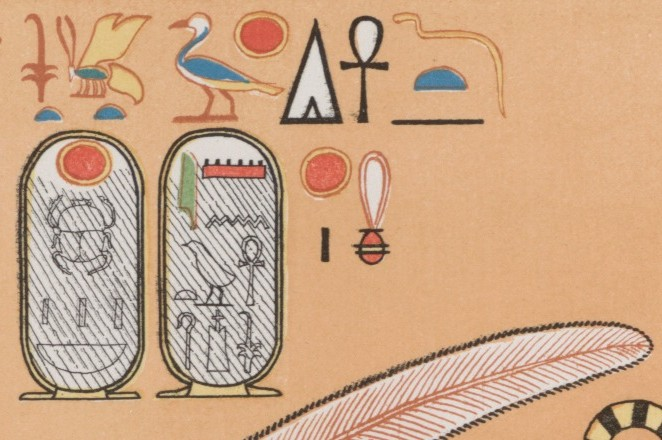
\includegraphics[width=0.8\textwidth]{images/img1.jpg}
			\caption{\cite{NYC:Ernst_1}}
			\label{fig:1}
		\end{figure}

		The hieroglyphs enclosed in the cartouche are obviously written vertically, while the rest is written horizontally. To figure out in what direction these hieroglyphs are read, pay close attention into which direction they are facing. 

		If you look, for example, at the goose, you can clearly see that it is facing to the left; same with the snake. You can therefore make the correct assumption that this text should be read from left to right. 

		Let us now look at the other inscription, namely Figure~\ref{fig:2}.

		\begin{figure}
			\centering
			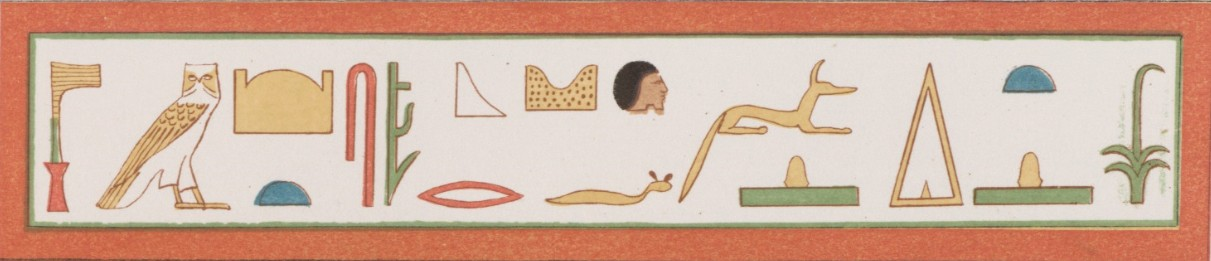
\includegraphics[width=0.8\textwidth]{images/img2.jpg}
			\caption{\cite{NYC:Ernst_Grab54}}
			\label{fig:2}
		\end{figure}

		Once again, look closely at the faces and the animals; what direction are they looking towards? Look, for instance, at the jackal hieroglyph \begin{hieroglyph}{\leavevmode \rightleft\HwordSpace
\loneSign{\Aca GE/47/}\HwordSpace
\leftright}\end{hieroglyph}\footnote{In this case, this sign is actually referring to the god Anubis.}; as you can clearly see, it is facing the right and thus you can be certain that — since you should always read into the hieroglyphs — this text should be read from right to left. Also remember that you should always read the top hieroglyphs first, thus reading it in the following order: \begin{hieroglyph}{\leavevmode \rightleft\HwordSpace
\loneSign{\Aca GR/35/}\HinterSignsSpace
\loneSign{\Aca GE/47/}\HinterSignsSpace
\loneSign{\Aca GX/40/}\HinterSignsSpace
\loneSign{\Aca GR/35/}\HinterSignsSpace
\loneSign{\Aca GX/32/}\HinterSignsSpace
\loneSign{\Aca GM/54/}\HwordSpace
\leftright}\end{hieroglyph}\footnote{This is only partly correct, since \begin{hieroglyph}{\leavevmode \rightleft\HwordSpace
\loneSign{\Aca GM/54/}\HinterSignsSpace
\Cadrat{\CadratLineI{\Aca GX/32/}\CadratLine{\Aca GR/35/}}\HinterSignsSpace
\loneSign{\Aca GX/40/}\HwordSpace
\leftright}\end{hieroglyph} is actually read as if it were written as \begin{hieroglyph}{\leavevmode \rightleft\HwordSpace
\loneSign{\Aca GR/35/}\HinterSignsSpace
\loneSign{\Aca GX/40/}\HinterSignsSpace
\loneSign{\Aca GM/54/}\HinterSignsSpace
\loneSign{\Aca GX/32/}\HwordSpace
\leftright}\end{hieroglyph}; this is because of what is known as honorific transposition which I will be covering more in-depth later.}. You can also easily see that writing the text as \begin{hieroglyph}{\leavevmode \rightleft\HwordSpace
\loneSign{\Aca GM/54/}\HinterSignsSpace
\Cadrat{\CadratLineI{\Aca GX/32/}\CadratLine{\Aca GR/35/}}\HinterSignsSpace
\loneSign{\Aca GX/40/}\HinterSignsSpace
\Cadrat{\CadratLineI{\Aca GE/47/}\negAROBvspace\negAROBvspace\negAROBvspace\negAROBvspace\CadratLine{{\Hsmaller\Aca GR/35/}}}\HinterSignsSpace
\leftright}\end{hieroglyph} rather than \begin{hieroglyph}{\leavevmode \rightleft\HwordSpace
\loneSign{\Aca GR/35/}\HinterSignsSpace
\loneSign{\Aca GE/47/}\HinterSignsSpace
\loneSign{\Aca GX/40/}\HinterSignsSpace
\loneSign{\Aca GR/35/}\HinterSignsSpace
\loneSign{\Aca GX/32/}\HinterSignsSpace
\loneSign{\Aca GM/54/}\HwordSpace
\leftright}\end{hieroglyph} not only saves space, but makes it look a lot more appealing.
		We will be referring back to these inscriptions later on.

\chapter*{The two varieties}
	\markboth{The two varieties}{The two varieties}
		\addcontentsline{toc}{chapter}{The two varieties}

		I would like to begin by covering the two different varieties of hieroglyphs, both of which being further divided into sub-groups — something you may have already realised by reading the previous parts. The first and easiest part of learning the Egyptian hieroglyphic script is the phonetic variety of hieroglyphs; these are those types of hieroglyphs that, as the name would already suggest, refer to a particular sound or group of sounds in the language. The phonetic hieroglyphs can be further divided into uni-, bi- and trilateral symbols.

		Unilateral glyphs are those that refer to only one sound, such as the symbol \begin{hieroglyph}{\leavevmode \loneSign{\Aca GS/63/}}\end{hieroglyph} which refers to the sound “s” and that we have already met before. 
		
		Bilateral symbols are ones that represent two sounds; this is actually not too strange for those who speak English, since many English letters represent two sounds. An example for this is the letter “i”; if you say the letter “i” on its own, you will, in actuality, be saying “ah-ee” which in reality are two different sounds. The same applies to Egyptian hieroglyphics. There are a great number of hieroglyphics that represent two sounds, such as the hieroglyph \begin{hieroglyph}{\leavevmode \loneSign{\Aca GO/32/}}\end{hieroglyph} — representing the sound sequence \textit{pr} — which we, too, have met previously.

		Trilaterals are, thus, those hieroglyphs that represent three sounds; an example for a trilateral hieroglyph is \begin{hieroglyph}{\leavevmode \loneSign{\Aca GR/39/}}\end{hieroglyph} — representing the sound sequence \textit{nṯr} — which can also, with a vertical stroke added onto it, have the meaning of “God”.

		The second, and frankly more difficult, variety of hieroglyphs is the logographic variety. Logographic hieroglyphs are ones that, unlike the phonetic ones, do not refer to a specific sound and instead refer to a concept or idea. 

		This, too, is not a foreign concept for speakers of the English language; take, for instance, a symbol commonly seen on electronic devices: ⏻. You are surely aware of its meaning and purpose — it will either start or shut-down your device — but it is not a letter as such, unlike “a”. It is a symbol that can be used cross-linguistically and still be understood; if you, instead, labelled the power button with an English word, it would only be understood by those that speak the language.

		English-speakers might call it “power button”, while German speakers may refer to it as “An-/Aus-Schalter”. Logographic hieroglyphs — which can also be referred to as Ideograms — work the same way. Instead of representing a sound — or a series of them —, they instead represent a concept, such as the previously mentioned symbol which represents the concept of a house: \begin{hieroglyph}{\leavevmode \Cadrat{\CadratLineI{\Aca GO/32/}\CadratLine{\Aca GZ/32/}}}\end{hieroglyph}.

		However, these ideographic symbols do not frequently stand on their own; instead, they are usually used to further specify the meaning of a word — they are then referred to as determinatives. A determinative may be used to avoid ambiguity or to aid in the reading of an unknown word. Unfortunately, there are no examples of this in the English language; we can, however, easily create one. Take, for instance, the English word “son”. Since Egyptian does not generally write its vowels, this would be written as “sn” in Egyptian, thus making it difficult to distinguish between “son” and “sun”. Egyptian avoids this problem by placing a determinative behind the word as such: —

    \begin{quote}
      son → sn → sn\begin{hieroglyph}{\leavevmode \loneSign{\Aca GA/32/}}\end{hieroglyph}; here, the picture of a male human being is added to clarify the meaning of this word as “son”.

      sun → sn → sn\begin{hieroglyph}{\leavevmode \loneSign{\Aca GN/36/}}\end{hieroglyph}; here we added the simplified drawing of the Sun in order to be able to distinguish is from the word “son” and to clarify that we are referring to the Sun instead.
    \end{quote}

    This is done frequently in Egyptian and there exist scores of other such determinatives; the meaning of many of them often being quite difficult to guess. Please note that determinatives do not actually influence the pronunciation of a word. Their sole purpose is to aid in the reading of words and to avoid ambiguity.

		Let us take a quick look at Thoth: \begin{hieroglyph}{\leavevmode \Cadrat{\CadratLineI{\Aca GG/59/}\CadratLine{\LoneHorizontalLine{\Aca GX/32/\hfill\Aca GZ/37/}}}\HinterSignsSpace
\loneSign{\Aca GC/34/}}\end{hieroglyph}. The first symbol\footnote{Remember to read into the hieroglyphs and from top to bottom. Thus, the first symbol, in this case, is the symbol on the top left.} is a determinative for Thoth, the following two symbols are phonetic symbols representing the sounds “t” and “y” and the last hieroglyph is yet another determinative. 
		
		A determinative can also help distinguishing between words such as \begin{hieroglyph}{\leavevmode \Cadrat{\CadratLineI{\Aca GO/32/}\CadratLine{\Aca GX/32/}}\HinterSignsSpace
\Cadrat{\CadratLineI{\Aca GD/52/}\CadratLine{\Aca GN/36/}}}\end{hieroglyph} (prt, one of the three Egyptian seasons) and \begin{hieroglyph}{\leavevmode \Cadrat{\CadratLineI{\Aca GO/32/}\CadratLine{\Aca GX/32/}}\HinterSignsSpace
\Cadrat{\CadratLineI{\Aca GD/52/}\CadratLine{\Aca GD/88/}}}\end{hieroglyph} (prt, procession); these two words have exactly the same pronunciation, so in order to distinguish one from the other, a determinative is added.

		You may be wondering how you can differentiate between a determinative and a regular logographic hieroglyph; and the answer is: a vertical stroke. If a hieroglyphic is being used as a logograph, a vertical stroke is — usually\footnote{With very common expressions it is often left out; it is also often left out if the scribe thought that leaving it would improve the text’s artistic value.} — added either underneath or next to the hieroglyphic sign. An example for this can be seen in Figure~\ref{fig:3}.

		\begin{figure}
			\centering
			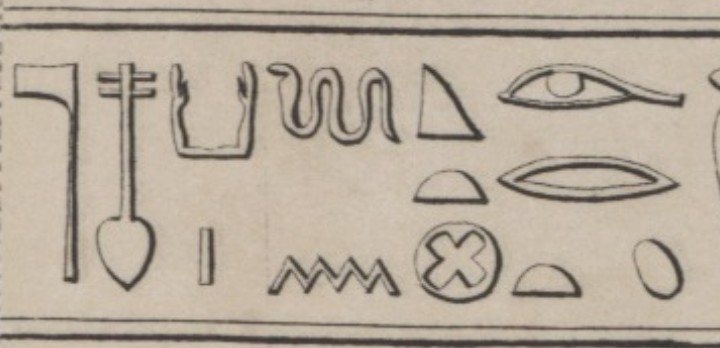
\includegraphics[width=0.8\textwidth]{images/img3.jpg}
			\caption{\cite{NYC:Ernst_Ptolost}}
			\label{fig:3}
		\end{figure}

		You can see the \begin{hieroglyph}{\leavevmode \Cadrat{\CadratLineI{\Aca GD/60/}\CadratLine{\Aca GZ/32/}}}\end{hieroglyph} hieroglyph has such a stroke underneath. Had it been written without said stroke, it might have been confused with the two-consonant sign “k\AHiero”; in addition, not adding the stroke would have resulted in a less pleasing-looking text — at least to the Egyptians\footnote{This is what it would have looked like without the stroke: \begin{hieroglyph}{\leavevmode \loneSign{\Aca GR/39/}\HinterSignsSpace
\loneSign{\Aca GF/66/}\HinterSignsSpace
\loneSign{\Aca GD/60/}\HinterSignsSpace
\Cadrat{\CadratLineI{\Aca GI/41/}\CadratLine{\Aca GN/66/}}}\end{hieroglyph}}.

		However, with the added sign there can be no doubt about this hieroglyph referring to the Ka. The Ka is part of what the Egyptians thought of as the soul\footnote{The Egyptian concept of “soul” is a lot different from ours. In Egyptian mythology, the “soul” on its own does not exist; instead, the soul consists of several unique parts.} and this particular part of the soul is what distinguishes a living being from a non-living being\footnote{A dead person would thus not possess the Ka while a living person would.}.

		Beware, however, that strokes like these may have other uses as well, such as denoting the plural\footnote{The plural of a word is that which refers to more than one: man → men} of words. Let us again take a look at the inscription discussed on page 17 which shows two of Tutankhamun’s names, one of which being \begin{hieroglyph}{\leavevmode \cartouche{\loneSign{\Aca GN/36/}\HinterSignsSpace
\loneSign{\Aca GL/32/}\HinterSignsSpace
\Cadrat{\CadratLineI{\Aca GZ/33/}\CadratLine{\Aca GV/61/}}}%
}\end{hieroglyph}\footnote{The name is transliterated as Nebkheperure and translated as “Lord of the Forms of Ra” — this is Tutankhamun’s Prænomen or Throne Name, preceded by \begin{hieroglyph}{\leavevmode \Cadrat{\CadratLineI{\Aca GM/54/}\CadratLine{\Aca GX/32/}}\HinterSignsSpace
\Cadrat{\CadratLineI{\Aca GL/33/}\CadratLine{\Aca GX/32/}}}\end{hieroglyph} meaning either “Dual King” or “King of Upper and Lower Egypt”.}.

		As you will notice, this name features three strokes next to each other; these are not, however, used to mark the usage of a particular sign as logographic. Instead, they are used to indicate the plural of the word \begin{hieroglyph}{\leavevmode \loneSign{\Aca GL/32/}}\end{hieroglyph}, meaning “form”. 

		Another very important thing to mention is another usage of unilateral hieroglyphs: Complementing bi- or trilaterals. This basically means that the Egyptians frequently added a unilateral hieroglyph where it would technically not be needed as the bi- or trilateral hieroglyph is already fulfilling that purpose.

		To explain this further, we will once again review the inscription on page \pageref{fig:1}; this time, however, we will be focussing on another of Tutankhamun’s names: \begin{hieroglyph}{\leavevmode \loneSign{\Aca GG/73/}\HinterSignsSpace
\negAROBspace\negAROBspace\Cadrat{\CadratLineI{\Aca GN/36/}\CadratLine{\HquarterSpace }}\HwordSpace
\cartouche{\loneSign{\Aca GM/48/}\HinterSignsSpace
\Cadrat{\CadratLineI{\Aca GY/36/}\CadratLine{\Aca GN/66/}}\HinterSignsSpace
\LoneHorizontalLine{\LoneHorizontalLine{\loneSign{\Aca GX/32/}\HinterSignsSpace
\loneSign{\Aca GG/77/}}\HinterSignsSpace
\negAROBspace\Cadrat{\CadratLineI{\Aca GX/32/}\CadratLine{\HquarterSpace }}}\HinterSignsSpace
\loneSign{\Aca GS/68/}\HwordSpace
\loneSign{\Aca GS/73/}\HinterSignsSpace
\loneSign{\Aca GO/59/}\HinterSignsSpace
\loneSign{\Aca GM/57/}}%
}\end{hieroglyph}\footnote{This is Tutankhamun’s Nomen, the name given to him at birth, which, as you can see in the picture, is preceded by \begin{hieroglyph}{\leavevmode \loneSign{\Aca GG/73/}\HinterSignsSpace
\negAROBspace\negAROBspace\Cadrat{\CadratLineI{\Aca GN/36/}\CadratLine{\HquarterSpace }}}\end{hieroglyph} meaning “Son of Ra”}. The first part of his name, , is generally transcribed as “jmn” (Amun). This is, however, not what has been written down, as \begin{hieroglyph}{\leavevmode \loneSign{\Aca GM/48/}\HinterSignsSpace
\Cadrat{\CadratLineI{\Aca GY/36/}\CadratLine{\Aca GN/66/}}}\end{hieroglyph} actually consists of the unilateral hieroglyph “j”, the bilateral “mn” and the unilateral “n”; thus, this part of his name is actually written as “jmn-n”.

		The reasoning behind doing this is twofold. On one hand, doing this aids reading and even those who were not experts in reading Egyptian hieroglyphs — which, back then, would have been the majority of the population — could easily guess that this name would have to be pronounced as “jmn”. On the other hand, adding a second hieroglyph can often increase the æsthetics of the word, as merely writing \begin{hieroglyph}{\leavevmode \loneSign{\Aca GM/48/}\HinterSignsSpace
\loneSign{\Aca GY/36/}}\end{hieroglyph} looks rather clunky and incomplete — at least to the Egyptians.

		As a rule of thumb, the last one or two sounds of a bi- or trilateral are usually written out as a unilateral beneath or next to the bi- or trilateral to complement it.\begin{hieroglyph}{\leavevmode \loneSign{\Aca GY/36/}}\end{hieroglyph} is one of most common bilateral symbols to receive a complement.

\chapter*{Unilaterals and Latinisation}
  \markboth{Unilaterals and Latinisation}{Unilaterals and Latinisation}
  \addcontentsline{toc}{chapter}{Unilaterals and Latinisation}

    We have just learnt about the different varieties of hieroglyphs and it is now time to actually start learning the unilateral variety of them. We will also be looking at how these symbols are transliterated into our alphabet.
    
    \begin{center}
      \begin{longtable}{p{0.18\linewidth} | p{0.23\linewidth} | p{0.45\linewidth}}
        Hieroglyph & Transliteration & Pronunciation \\ [0.5ex]
        \hline\hline
        \begin{hieroglyph}{\leavevmode \loneSign{\Aca GG/32/}}\end{hieroglyph} & \AHiero, A & short “a” as in “hat” \\
        \hline
        \begin{hieroglyph}{\leavevmode \loneSign{\Aca GM/48/}}\end{hieroglyph} & j & like “ee” or “ea” (heat, eat, beet) \\
        \hline
        \begin{hieroglyph}{\leavevmode \LoneHorizontalLine{\loneSign{\Aca GM/48/}\HinterSignsSpace
\loneSign{\Aca GM/48/}}}\end{hieroglyph}, \begin{hieroglyph}{\leavevmode \loneSign{\Aca GZ/37/}}\end{hieroglyph} & y & “
        or like “y” in “yet” \\
        \hline
        \begin{hieroglyph}{\leavevmode \loneSign{\Aca GD/69/}}\end{hieroglyph} & \aHiero, a & long “a” as in “bath” \\
        \hline
        \begin{hieroglyph}{\leavevmode \loneSign{\Aca GG/77/}}\end{hieroglyph}, \begin{hieroglyph}{\leavevmode \loneSign{\Aca GZ/40/}}\end{hieroglyph} & w & like “oo” as in “boot” \\
        \hline
        \begin{hieroglyph}{\leavevmode \loneSign{\Aca GD/92/}}\end{hieroglyph} & b & b as in “bed” \\
        \hline
        \begin{hieroglyph}{\leavevmode \loneSign{\Aca GQ/34/}}\end{hieroglyph} & p & p as in “pet” \\
        \hline
        \begin{hieroglyph}{\leavevmode \loneSign{\Aca GI/41/}}\end{hieroglyph} & f & f as in “foot“ \\
        \hline
        \begin{hieroglyph}{\leavevmode \loneSign{\Aca GG/50/}}\end{hieroglyph} & m & m as in “mouse“ \\
        \hline
        \begin{hieroglyph}{\leavevmode \loneSign{\Aca GN/66/}}\end{hieroglyph} & n & n as in “night“ \\
        \hline
        \begin{hieroglyph}{\leavevmode \loneSign{\Aca GD/52/}}\end{hieroglyph} & r & trilled r (like Spanish or Scottish English) \\
        \hline
        \begin{hieroglyph}{\leavevmode \loneSign{\Aca GO/35/}}\end{hieroglyph} & h & h as in “house“ \\
        \hline
        \begin{hieroglyph}{\leavevmode \loneSign{\Aca GV/59/}}\end{hieroglyph} & H, ḥ & h but pronounced further down in the throat (like panting) \\
        \hline
        \begin{hieroglyph}{\leavevmode \loneSign{\Aca GAa/32/}}\end{hieroglyph} & ḫ, x & like the “ch” in “Loch Ness”; Spanish “j”; German “ch”.\\
        \hline
        \begin{hieroglyph}{\leavevmode \loneSign{\Aca GF/63/}}\end{hieroglyph} & ẖ, X & like German “ch” in “ich”; like “h” in B.E. “hue”. \\
        \hline
        \begin{hieroglyph}{\leavevmode \loneSign{\Aca GS/63/}}\end{hieroglyph}, \begin{hieroglyph}{\leavevmode \loneSign{\Aca GO/65/}}\end{hieroglyph} & s, z & like “s” in “street” or like “z” in “zero” \\
        \hline
        \begin{hieroglyph}{\leavevmode \loneSign{\Aca GN/69/}}\end{hieroglyph} & š or S & like “sh” in “ship” \\
        \hline
        \begin{hieroglyph}{\leavevmode \loneSign{\Aca GN/60/}}\end{hieroglyph} & ḳ or q & like “k” but pronounced further down in the throat \\
        \hline
        \begin{hieroglyph}{\leavevmode \loneSign{\Aca GV/62/}}\end{hieroglyph} & k & like “k” in “kite” \\
        \hline
        \begin{hieroglyph}{\leavevmode \loneSign{\Aca GW/44/}}\end{hieroglyph} & g & like “g” in “get” \\
        \hline
        \begin{hieroglyph}{\leavevmode \loneSign{\Aca GX/32/}}\end{hieroglyph} & t & like “t” in “tube” \\
        \hline
        \begin{hieroglyph}{\leavevmode \loneSign{\Aca GV/44/}}\end{hieroglyph} & ṯ, T & like “tsh” or “tch” (hatch, satchel) \\
        \hline
        \begin{hieroglyph}{\leavevmode \loneSign{\Aca GD/79/}}\end{hieroglyph} & d & like “d” in “dark” \\
        \hline
        \begin{hieroglyph}{\leavevmode \loneSign{\Aca GX/32/}}\end{hieroglyph} & ḏ, D & like “j” in “jungle” \\
        \hline
      \end{longtable}
    \end{center}

    You may be wondering why there are occasionally two possible transliterations for the same hieroglyph. The reason behind this is that the second variety is used when special symbols, such as “ẖ”, are unavailable — a very common problem on computers. If you, for instance, wish to type hieroglyphs using the program JSesh, you are required to use the second transliteration (i.e S instead of š). This second type of transliteration is known as Manuel de Codage, or MdC for short, and it is the standard transliteration used for the Egyptian language when typing with your regular keyboard.

    You might, however, also ask yourself why there are different ways of writing the same sound. First of all, this should not surprise you, as English does something rather similar; what is, for example, the difference between the “c” and the “k” in the word “cake”? The answer is: there is no difference. Second of all, let us take a quick look at the three pairs hieroglyphs and find out what the differences between them are: —

    \begin{itemize}
			\item \begin{hieroglyph}{\leavevmode \loneSign{\Aca GS/63/}}\end{hieroglyph}, \begin{hieroglyph}{\leavevmode \loneSign{\Aca GO/65/}}\end{hieroglyph}. Originally, these two signs would have been pronounced differently, the first being “s” (as in “stop”) and the second being “z” (as in “zero”). Over time, however, these two sounds have into one and could be used interchangeably. The word \begin{hieroglyph}{\leavevmode \Cadrat{\CadratLineI{\Aca GZ/32/}\negAROBvspace\negAROBvspace\negAROBvspace\negAROBvspace\negAROBvspace\CadratLine{{\Hsmaller\Aca GG/73/}}}}\end{hieroglyph} can therefore be transcribed as either “s\AHiero” or “z\AHiero”.
			\item \begin{hieroglyph}{\leavevmode \LoneHorizontalLine{\loneSign{\Aca GM/48/}\HinterSignsSpace
\loneSign{\Aca GM/48/}}}\end{hieroglyph}, \begin{hieroglyph}{\leavevmode \loneSign{\Aca GZ/37/}}\end{hieroglyph}. The former is generally used inside of regular words and the latter is generally used as a grammatical ending or simply when it fits better.
			\item \begin{hieroglyph}{\leavevmode \loneSign{\Aca GG/77/}}\end{hieroglyph}, \begin{hieroglyph}{\leavevmode \loneSign{\Aca GZ/40/}}\end{hieroglyph}. See above.
    \end{itemize}

		The letters \begin{hieroglyph}{\leavevmode \loneSign{\Aca GN/66/}}\end{hieroglyph} and \begin{hieroglyph}{\leavevmode \loneSign{\Aca GG/50/}}\end{hieroglyph} could also be written, especially in later times, as \begin{hieroglyph}{\leavevmode \loneSign{\Aca GS/34/}}\end{hieroglyph} and \begin{hieroglyph}{\leavevmode \loneSign{\Aca GAa/43/}}\end{hieroglyph} respectively. We will, however, not be seeing these version too often.

		Another matter we should discuss is vowels\footnote{Such as “a”, “e”, “o” etc.}. You may have already realised that many of the vowels used in the English language have no equivalent unilateral hieroglyphic symbol. This is due to the fact that Egyptians generally ignored vowels altogether; this means that we are often required to “fill in the gaps”, so to speak. Consider, for example, the name \begin{hieroglyph}{\leavevmode \loneSign{\Aca GM/48/}\HinterSignsSpace
\Cadrat{\CadratLineI{\Aca GY/36/}\CadratLine{\Aca GN/66/}}}\end{hieroglyph}. It is written as “jmn”, yet Egyptologists pronounce it as if it were written with a vowel between the “m” and the “n”: “jm(e)n”. The reason for doing this is that saying “mn” is much more difficult than saying “men”.

		Therefore, you always add a vowel — Egyptological convention is to use an “e” — in-between consonants. Another example of this is the trilateral hieroglyph \begin{hieroglyph}{\leavevmode \loneSign{\Aca GR/39/}}\end{hieroglyph}; it is transcribed as “nṯr” but pronounced as “neṯer”. I would like to point out, however, that this is not how the Ancient Egyptians spoke and merely there to assist us so that we have an easier time pronouncing Ancient Egyptian words. 

		You should now be able to read the following, transliterated names of people and cities (to ease reading, names are inside an oval cartouche and cities inside a rectangular one; this is now how the Ancient Egyptians handled the matter and simply there so that it might be easier for you to recognise the names). This is the first exercise of this book, §1: —
		
		\begin{center}
			\begin{hieroglyph}{\leavevmode \cartouche{\loneSign{\Aca GG/50/}\HinterSignsSpace
\Cadrat{\CadratLineI{\Aca GD/52/}\CadratLine{\Aca GZ/37/}}}%
}\end{hieroglyph} \bigskip\linebreak\bigskip
			\begin{hieroglyph}{\leavevmode \chateau{\Cadrat{\CadratLineI{\Aca GN/66/}\CadratLine{\Aca GG/77/}}\HinterSignsSpace
\loneSign{\Aca GZ/37/}\HinterSignsSpace
\Cadrat{\CadratLineI{\Aca GD/52/}\CadratLine{\Aca GV/62/}}}%
}\end{hieroglyph} \linebreak\bigskip
			\begin{hieroglyph}{\leavevmode \chateau{\Cadrat{\CadratLineI{\Aca GO/65/}\CadratLine{\Aca GZ/37/}}\HinterSignsSpace
\loneSign{\Aca GG/32/}\HinterSignsSpace
\Cadrat{\CadratLineI{\Aca GX/32/}\CadratLine{\Aca GD/52/}}}%
}\end{hieroglyph} \linebreak\bigskip
			\begin{hieroglyph}{\leavevmode \cartouche{\loneSign{\Aca GG/50/}\HinterSignsSpace
\loneSign{\Aca GG/32/}\HinterSignsSpace
\Cadrat{\CadratLineI{\Aca GD/52/}\CadratLine{\Aca GI/41/}}\HinterSignsSpace
\Cadrat{\CadratLineI{\Aca GZ/37/}\CadratLine{\Aca GN/66/}}}%
}\end{hieroglyph} \linebreak\bigskip
			\begin{hieroglyph}{\leavevmode \chateau{\loneSign{\Aca GG/77/}\HinterSignsSpace
\loneSign{\Aca GG/32/}\HinterSignsSpace
\Cadrat{\CadratLineI{\Aca GN/69/}\CadratLine{\Aca GZ/37/}}\HinterSignsSpace
\Cadrat{\CadratLineI{\Aca GN/66/}\CadratLine{\Aca GW/44/}}\HinterSignsSpace
\Cadrat{\CadratLineI{\Aca GX/32/}\CadratLine{\Aca GZ/37/}}\HinterSignsSpace
\loneSign{\Aca GS/34/}}%
}\end{hieroglyph} \linebreak
		\end{center}

		Remember that many vowels are not written or are written differently. Also note that there is no “l” in Ancient Egyptian; it will often be replaced by an “r”i.
		You should also be able to easily do exercise §2 by reading the following name: —
      \begin{center}
        \EnColonne[1.2\Htm]{
          \begin{hieroglyph}{\leavevmode \cartouche{\loneSign{\Aca GAa/32/}\HinterSignsSpace
\loneSign{\Aca GI/41/}\HinterSignsSpace
\loneSign{\Aca GG/77/}}%
}\end{hieroglyph}
        }
      \end{center}
    For the solutions to these exercises, please go to page \pageref{solutions}.

\chapter*{Bi- and trilaterals}
  \markboth{Bi- and trilaterals}{Bi- and trilaterals}
  \addcontentsline{toc}{chapter}{Bi- and trilaterals}

    The list of bi- and trilateral symbols is rather extensive and listing the entirety of them here would not only be rather difficult but also unnecessary; this is because only a couple of dozen of these were actually in common use and we will therefore be learning them as we go along. 
    We have, however, already met the following dozen common tri- and bilateral hieroglyphic signs: —

    \begin{center}
      \begin{longtable}{p{0.45\linewidth} | p{0.45\linewidth}}
        Bi- or trilateral hieroglyph & Transliteration \\ [0.5ex]
        \hline\hline
        \begin{hieroglyph}{\leavevmode \loneSign{\Aca GX/40/}}\end{hieroglyph} & dj \\
        \hline
        \begin{hieroglyph}{\leavevmode \loneSign{\Aca GD/60/}}\end{hieroglyph} & k\AHiero \\
        \hline
        \begin{hieroglyph}{\leavevmode \loneSign{\Aca GY/36/}}\end{hieroglyph} & mn \\
        \hline
        \begin{hieroglyph}{\leavevmode \loneSign{\Aca GV/61/}}\end{hieroglyph} & nb \\
        \hline
        \begin{hieroglyph}{\leavevmode \loneSign{\Aca GO/32/}}\end{hieroglyph} & pr \\
        \hline
        \begin{hieroglyph}{\leavevmode \loneSign{\Aca GN/36/}}\end{hieroglyph} & r\aHiero \\
        \hline
        \begin{hieroglyph}{\leavevmode \loneSign{\Aca GM/54/}}\end{hieroglyph} & sw \\
        \hline
        \begin{hieroglyph}{\leavevmode \loneSign{\Aca GG/73/}}\end{hieroglyph} & z\AHiero, s\AHiero \\
        \hline
        \begin{hieroglyph}{\leavevmode \loneSign{\Aca GS/68/}}\end{hieroglyph} & \aHiero\xHiero\\
        \hline
        \begin{hieroglyph}{\leavevmode \loneSign{\Aca GR/35/}}\end{hieroglyph} & \HHiero tp \\
        \hline
        \begin{hieroglyph}{\leavevmode \loneSign{\Aca GF/66/}}\end{hieroglyph} & nfr \\
        \hline
        \begin{hieroglyph}{\leavevmode \loneSign{\Aca GL/32/}}\end{hieroglyph} & \xHiero pr \\
        \hline
      \end{longtable}
    \end{center}

    For a more complete list of bi- and trilateral hieroglyphs, take a look at the appendix on page \pageref{bitri}.

    Learning these will give you a good basis for understanding the upcoming inscriptions. Please also note that these bi- and trilateral hieroglyphic symbols can often denote not only a sound-sequence but also an entire word or concept; this is generally done in very common formulæ, such as \begin{hieroglyph}{\leavevmode \loneSign{\Aca GM/54/}\HinterSignsSpace
\Cadrat{\CadratLineI{\Aca GX/32/}\CadratLine{\Aca GR/35/}}\HinterSignsSpace
\loneSign{\Aca GX/40/}}\end{hieroglyph} (ḥtp-ḏj-nswt). The word \textit{ḥtp} would, for example, usually be written as when standing on its own (i.e. with two unilateral hieroglyphs added onto it). We will be learning more about that in Not writing sounds on page ENTER PAGE.

  \chapter*{Determinatives and ideograms}
    \markboth{Determinatives and ideograms}{Determinatives and ideograms}
    \addcontentsline{toc}{chapter}{Determinatives and ideograms}
    The amount of determinatives in the Egyptian language is staggering; not only that, they also often have more than one meaning and it will hence be impossible to list all potential meanings of every single one of the determinatives in this book. We will thus only concern ourselves with determinatives as soon as we see one in use.

		Ideograms, unlike determinatives which often have several meanings, almost always refer to only one concept or idea or variations thereof. It is therefore much easier to create a list of these and their possible translation, especially since only a handful of rather common expressions are conveyed using ideograms. Let us therefore take a look at a few of the most commonly used ones, their transliteration and their meaning: —

    \begin{center}
      \begin{longtable}{p{0.18\linewidth} | p{0.23\linewidth} | p{0.45\linewidth}}
        Ideogram & Transliteration & Meaning \\ [0.5ex]
        \hline\hline
        \begin{hieroglyph}{\leavevmode \Cadrat{\CadratLineI{\Aca GF/65/}\CadratLine{\Aca GZ/32/}}}\end{hieroglyph} & jb & heart \\
        \hline
				\begin{hieroglyph}{\leavevmode \loneSign{\Aca GA/32/}}\end{hieroglyph} & j & me, I (usually used after verbs) \\
        \hline
				\begin{hieroglyph}{\leavevmode \LoneHorizontalLine{\loneSign{\Aca GR/39/}\HinterSignsSpace
\loneSign{\Aca GZ/32/}}}\end{hieroglyph} & n\THiero r & god \\
        \hline
				\begin{hieroglyph}{\leavevmode \Cadrat{\CadratLineI{\Aca GO/80/}\CadratLine{\LoneHorizontalLine{\Aca GX/32/\hfill\Aca GZ/32/}}}}\end{hieroglyph} & nwt & town \\
        \hline
				\begin{hieroglyph}{\leavevmode \Cadrat{\CadratLineI{\Aca GO/32/}\CadratLine{\Aca GZ/32/}}}\end{hieroglyph} & pr & house \\
        \hline
				\begin{hieroglyph}{\leavevmode \Cadrat{\CadratLineI{\Aca GN/36/}\CadratLine{\Aca GZ/32/}}}\end{hieroglyph} & r\aHiero & sun \\
        \hline
				\begin{hieroglyph}{\leavevmode \loneSign{\Aca GM/35/}\HinterSignsSpace
\Cadrat{\CadratLineI{\Aca GX/32/}\CadratLine{\Aca GZ/32/}}}\end{hieroglyph} & rnpt & year \\
        \hline
				\begin{hieroglyph}{\leavevmode \loneSign{\Aca GQ/32/}\HinterSignsSpace
\Cadrat{\CadratLineI{\Aca GX/32/}\CadratLine{\Aca GO/32/}}}\end{hieroglyph} & st & palace, throne \\
        \hline
				\begin{hieroglyph}{\leavevmode \Cadrat{\CadratLineI{\Aca GN/47/}\CadratLine{\LoneHorizontalLine{\Aca GN/54/\hfill\Aca GZ/32/}}}}\end{hieroglyph} & t\AHiero & land, country \\
        \hline
				\begin{hieroglyph}{\leavevmode \Cadrat{\CadratLineI{\Aca GN/62/}\CadratLine{\LoneHorizontalLine{\Aca GX/32/\hfill\Aca GZ/32/}}}}\end{hieroglyph} & w\AHiero t & street \\
        \hline
				\begin{hieroglyph}{\leavevmode \Cadrat{\CadratLineI{\Aca GZ/32/}\negAROBvspace\negAROBvspace\negAROBvspace\negAROBvspace\negAROBvspace\CadratLine{{\Hsmaller\Aca GG/73/}}}}\end{hieroglyph} & z\AHiero & son \\
				\hline
      \end{longtable}
    \end{center}

		Please bear in mind, however, that these are not the only spellings that were possible; Ancient Egyptian spelling was rather flexible, these are simply some of the most commonly used spellings but in no way the only spellings.


  \chapter*{Numbers and dates}
    \markboth{Numbers and dates}{Numbers and dates}
    \addcontentsline{toc}{chapter}{Numbers and dates}

		The Egyptians also had their own, unique way of writing dates and numbers — the latter functioning similar to Roman numerals. Different numerical hieroglyphs exist, each one representing one of the different powers of ten: 1, 10, 100,  1 000, 10 000, 100 000 and 1 000 000. These can, when combined, form any other number except for the number 0. Here is a short overview of the Egyptian numerals: —

    \begin{center}
      \begin{longtable}{p{0.45\linewidth} | p{0.45\linewidth}}
        Egyptian numeral & English numeral \\ [0.5ex]
        \hline\hline
        \begin{hieroglyph}{\leavevmode \loneSign{\Aca GZ/32/}}\end{hieroglyph} & 1 \\
        \hline
        \begin{hieroglyph}{\leavevmode \loneSign{\Aca GV/51/}}\end{hieroglyph} & 10 \\
        \hline
        \begin{hieroglyph}{\leavevmode \loneSign{\Aca GV/32/}}\end{hieroglyph} & 100 \\
        \hline
        \begin{hieroglyph}{\leavevmode \loneSign{\Aca GM/43/}}\end{hieroglyph} & 1,000 \\
        \hline
        \begin{hieroglyph}{\leavevmode \loneSign{\Aca GD/84/}}\end{hieroglyph} & 10,000 \\
        \hline
        \begin{hieroglyph}{\leavevmode \loneSign{\Aca GI/40/}}\end{hieroglyph} & 100,000 \\
        \hline
        \begin{hieroglyph}{\leavevmode \loneSign{\Aca GC/42/}}\end{hieroglyph} & 1,000,000 \\
        \hline
      \end{longtable}
    \end{center}

		Forming numbers such as “13” would therefore require the usage of one of the symbols representing “10” and three symbols representing “1” like this: \begin{hieroglyph}{\leavevmode \Cadrat{\CadratLineI{\Aca GV/51/}\CadratLine{\LoneHorizontalLine{\Aca GZ/32/\hfill\Aca GZ/32/\hfill\Aca GZ/32/}}}}\end{hieroglyph}.

		  \begin{wrapfigure}{R}{0.45\textwidth}
				\centering
				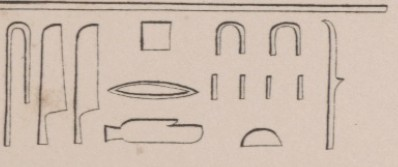
\includegraphics[width=0.4\textwidth]{images/img5.jpg}
				\caption{The number 24}
				\cite{NYC:Ernst_Ptolost}
			\end{wrapfigure}

			Egyptian years work quite differently from ours. Unlike the Gregorian Calendar — the calendar we use —, which is based on the supposed year of birth of Jesus of Nazareth1, the 1st year of the Egyptian calendar generally fell on the year of inauguration of the then reigning king.

			You can imagine it as follows: The coronation of Queen Elizabeth II. was in the year 1953; what the Egyptians then did was to use this year as their year 1. Therefore, the Gregorian year 2019 would turn into the Elizabethan year 65. Let us then suppose that Charles Philip Arthur George will be coronated in the year 2020; the year 2020 would then become the new year 1 and thus, the  Gregorian year 2025 would be the 5th year under the reign of Charles. 

			The Egyptians generally worded it thus: “Regnal year X under [the rule of] his majesty, the King X”, which was mostly written in the following manner: —

			\begin{quote}
				\begin{hieroglyph}{\leavevmode \loneSign{\Aca GM/35/}\HinterSignsSpace
\Cadrat{\CadratLineI{\Aca GX/32/}\CadratLine{\Aca GO/81/}}\HinterSignsSpace
\Cadrat{\CadratLineI{\Aca GAa/32/}\CadratLine{\Aca GD/52/}}\HinterSignsSpace
\loneSign{\Aca GU/70/}\HinterSignsSpace
\Cadrat{\CadratLineI{\Aca GZ/32/}\CadratLine{\Aca GN/66/}}}\end{hieroglyph}
				\newline
				\textit{rnpt-\HHiero sb \xHiero r \HHiero m n}
			\end{quote}

			Let us dissect this expression before we continue. The first part of the expression, \begin{hieroglyph}{\leavevmode \loneSign{\Aca GM/35/}\HinterSignsSpace
\Cadrat{\CadratLineI{\Aca GX/32/}\CadratLine{\Aca GO/81/}}}\end{hieroglyph} (rnpt-ḥsb), literally translates as “The year of counting”; nevertheless, it is largely translated as “regnal year”, which is the translation I will be using as well.

			The second part, \begin{hieroglyph}{\leavevmode \Cadrat{\CadratLineI{\Aca GAa/32/}\CadratLine{\Aca GD/52/}}}\end{hieroglyph} (ḫr), is a preposition that, in this case, is translated as “under” which can be understood as a shortening of “under the rule / reign”.

			The third part, \begin{hieroglyph}{\leavevmode \LoneHorizontalLine{\loneSign{\Aca GU/70/}\HinterSignsSpace
\loneSign{\Aca GZ/32/}}}\end{hieroglyph} (ḥm), is, in this particular instance, generally translated as “(his) Majesty”.

			The fourth and last part of this expression, \begin{hieroglyph}{\leavevmode \loneSign{\Aca GN/66/}}\end{hieroglyph} (n), marks what is known as an “indirect genitive”; this, however, sounds more complicated than it actually is, since this can be easily translated as meaning “of”.
			Here an example of the full expression from the reign of Intef (shortened for your convenience): —

			\begin{quote}
				\begin{hieroglyph}{\leavevmode \loneSign{\Aca GM/35/}\HinterSignsSpace
\Cadrat{\CadratLineI{\Aca GX/32/}\CadratLine{\Aca GZ/32/}\CadratLine{\Aca GZ/32/\hfill\Aca GZ/32/\hfill\Aca GZ/32/}}\HinterSignsSpace
\Cadrat{\CadratLineI{\Aca GAa/32/}\CadratLine{\Aca GD/52/}}\HinterSignsSpace
\loneSign{\Aca GU/70/}\HinterSignsSpace
\Cadrat{\CadratLineI{\Aca GZ/32/}\CadratLine{\Aca GN/66/}}\HinterSignsSpace
\HfullSpace \HinterSignsSpace
\Cadrat{\CadratLineI{\Aca GM/54/}\CadratLine{\Aca GX/32/}}\HinterSignsSpace
\Cadrat{\CadratLineI{\Aca GL/33/}\CadratLine{\Aca GX/32/}}\HinterSignsSpace
\cartouche{\loneSign{\Aca GG/73/}\HinterSignsSpace
\negAROBspace\negAROBspace\Cadrat{\CadratLineI{\Aca GN/36/}\CadratLine{\HquarterSpace }}\HwordSpace
\loneSign{\Aca GW/58/}\HinterSignsSpace
\Cadrat{\CadratLineI{\Aca GN/66/}\CadratLine{\Aca GX/32/}\CadratLine{\Aca GI/41/}}}%
}\end{hieroglyph}
				\newline
				\textit{rnpt 4 \xHiero r \HHiero m (n)swt-bjtj jnj-jt.f}
			\end{quote}





	%%% APPENDIX %%%
	\part*{Appendix}
  \chapter*{List of bilateral hieroglyphs}
    \markboth{List of bilateral hieroglyphs}{List of bilateral hieroglyphs}
    \addcontentsline{toc}{chapter}{List of bilateral hieroglyphs}
    \label{bitri}

  \chapter*{List of trilateral hieroglyphs}
    \markboth{List of trilateral hieroglyphs}{List of trilateral hieroglyphs}
    \addcontentsline{toc}{chapter}{List of trilateral hieroglyphs}
    \newpage

  \chapter*{Solutions to exercises}
    \markboth{Solutions to exercises}{Solutions to exercises}
    \addcontentsline{toc}{chapter}{Solutions to exercises}
    \label{solutions}
    \newpage

		\markboth{Bibliography}{Bibliography}
		\addcontentsline{toc}{part}{Bibliography}
		\newpage
		\printbibliography
\end{document}
